\documentclass[twoside]{book}

% Packages required by doxygen
\usepackage{fixltx2e}
\usepackage{calc}
\usepackage{doxygen}
\usepackage[export]{adjustbox} % also loads graphicx
\usepackage{graphicx}
\usepackage[utf8]{inputenc}
\usepackage{makeidx}
\usepackage{multicol}
\usepackage{multirow}
\PassOptionsToPackage{warn}{textcomp}
\usepackage{textcomp}
\usepackage[nointegrals]{wasysym}
\usepackage[table]{xcolor}

% Font selection
\usepackage[T1]{fontenc}
\usepackage[scaled=.90]{helvet}
\usepackage{courier}
\usepackage{amssymb}
\usepackage{sectsty}
\renewcommand{\familydefault}{\sfdefault}
\allsectionsfont{%
  \fontseries{bc}\selectfont%
  \color{darkgray}%
}
\renewcommand{\DoxyLabelFont}{%
  \fontseries{bc}\selectfont%
  \color{darkgray}%
}
\newcommand{\+}{\discretionary{\mbox{\scriptsize$\hookleftarrow$}}{}{}}

% Page & text layout
\usepackage{geometry}
\geometry{%
  a4paper,%
  top=2.5cm,%
  bottom=2.5cm,%
  left=2.5cm,%
  right=2.5cm%
}
\tolerance=750
\hfuzz=15pt
\hbadness=750
\setlength{\emergencystretch}{15pt}
\setlength{\parindent}{0cm}
\setlength{\parskip}{3ex plus 2ex minus 2ex}
\makeatletter
\renewcommand{\paragraph}{%
  \@startsection{paragraph}{4}{0ex}{-1.0ex}{1.0ex}{%
    \normalfont\normalsize\bfseries\SS@parafont%
  }%
}
\renewcommand{\subparagraph}{%
  \@startsection{subparagraph}{5}{0ex}{-1.0ex}{1.0ex}{%
    \normalfont\normalsize\bfseries\SS@subparafont%
  }%
}
\makeatother

% Headers & footers
\usepackage{fancyhdr}
\pagestyle{fancyplain}
\fancyhead[LE]{\fancyplain{}{\bfseries\thepage}}
\fancyhead[CE]{\fancyplain{}{}}
\fancyhead[RE]{\fancyplain{}{\bfseries\leftmark}}
\fancyhead[LO]{\fancyplain{}{\bfseries\rightmark}}
\fancyhead[CO]{\fancyplain{}{}}
\fancyhead[RO]{\fancyplain{}{\bfseries\thepage}}
\fancyfoot[LE]{\fancyplain{}{}}
\fancyfoot[CE]{\fancyplain{}{}}
\fancyfoot[RE]{\fancyplain{}{\bfseries\scriptsize Generated by Doxygen }}
\fancyfoot[LO]{\fancyplain{}{\bfseries\scriptsize Generated by Doxygen }}
\fancyfoot[CO]{\fancyplain{}{}}
\fancyfoot[RO]{\fancyplain{}{}}
\renewcommand{\footrulewidth}{0.4pt}
\renewcommand{\chaptermark}[1]{%
  \markboth{#1}{}%
}
\renewcommand{\sectionmark}[1]{%
  \markright{\thesection\ #1}%
}

% Indices & bibliography
\usepackage{natbib}
\usepackage[titles]{tocloft}
\setcounter{tocdepth}{3}
\setcounter{secnumdepth}{5}
\makeindex

% Hyperlinks (required, but should be loaded last)
\usepackage{ifpdf}
\ifpdf
  \usepackage[pdftex,pagebackref=true]{hyperref}
\else
  \usepackage[ps2pdf,pagebackref=true]{hyperref}
\fi
\hypersetup{%
  colorlinks=true,%
  linkcolor=blue,%
  citecolor=blue,%
  unicode%
}

% Custom commands
\newcommand{\clearemptydoublepage}{%
  \newpage{\pagestyle{empty}\cleardoublepage}%
}

\usepackage{caption}
\captionsetup{labelsep=space,justification=centering,font={bf},singlelinecheck=off,skip=4pt,position=top}

%===== C O N T E N T S =====

\begin{document}

% Titlepage & ToC
\hypersetup{pageanchor=false,
             bookmarksnumbered=true,
             pdfencoding=unicode
            }
\pagenumbering{roman}
\begin{titlepage}
\vspace*{7cm}
\begin{center}%
{\Large My Project }\\
\vspace*{1cm}
{\large Generated by Doxygen 1.8.11}\\
\end{center}
\end{titlepage}
\clearemptydoublepage
\tableofcontents
\clearemptydoublepage
\pagenumbering{arabic}
\hypersetup{pageanchor=true}

%--- Begin generated contents ---
\chapter{R\+E\+A\+D\+ME}
\label{md_README}
\hypertarget{md_README}{}
Приложение для конвертации файлов типа csv и sqllite. 
\chapter{Hierarchical Index}
\section{Class Hierarchy}
This inheritance list is sorted roughly, but not completely, alphabetically\+:\begin{DoxyCompactList}
\item Q\+Abstract\+Table\+Model\begin{DoxyCompactList}
\item \contentsline{section}{B\+D\+Data}{\pageref{classBDData}}{}
\end{DoxyCompactList}
\item Q\+Main\+Window\begin{DoxyCompactList}
\item \contentsline{section}{Main\+Window}{\pageref{classMainWindow}}{}
\end{DoxyCompactList}
\end{DoxyCompactList}

\chapter{Class Index}
\section{Class List}
Here are the classes, structs, unions and interfaces with brief descriptions\+:\begin{DoxyCompactList}
\item\contentsline{section}{\hyperlink{classBDData}{B\+D\+Data} \\*The \hyperlink{classBDData}{B\+D\+Data} class }{\pageref{classBDData}}{}
\item\contentsline{section}{\hyperlink{classMainWindow}{Main\+Window} }{\pageref{classMainWindow}}{}
\end{DoxyCompactList}

\chapter{Class Documentation}
\hypertarget{classBDData}{}\section{B\+D\+Data Class Reference}
\label{classBDData}\index{B\+D\+Data@{B\+D\+Data}}


The \hyperlink{classBDData}{B\+D\+Data} class.  




{\ttfamily \#include $<$bddata.\+h$>$}



Inheritance diagram for B\+D\+Data\+:\nopagebreak
\begin{figure}[H]
\begin{center}
\leavevmode
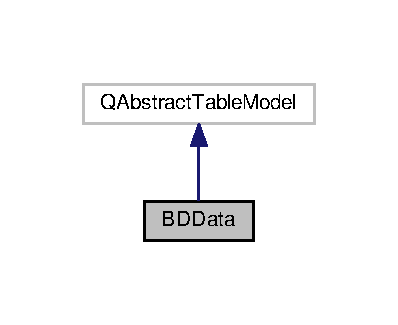
\includegraphics[width=191pt]{classBDData__inherit__graph}
\end{center}
\end{figure}


Collaboration diagram for B\+D\+Data\+:\nopagebreak
\begin{figure}[H]
\begin{center}
\leavevmode
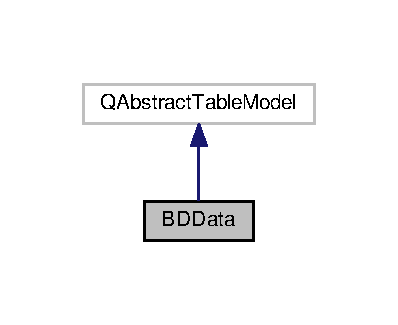
\includegraphics[width=191pt]{classBDData__coll__graph}
\end{center}
\end{figure}
\subsection*{Public Member Functions}
\begin{DoxyCompactItemize}
\item 
\hyperlink{classBDData_a74a3f4246018e4c20f7af94a92f6933d}{B\+D\+Data} (Q\+Object $\ast$parent=nullptr)
\begin{DoxyCompactList}\small\item\em \hyperlink{classBDData}{B\+D\+Data} конструктор по-\/умолчанию \end{DoxyCompactList}\item 
\hyperlink{classBDData_a7740b599addc9dc7cbcaa6e91bf9b494}{B\+D\+Data} (Q\+List$<$ Q\+String $>$ column\+\_\+name, Q\+List$<$ Q\+String $>$ data\+\_\+type, Q\+List$<$ Q\+List$<$ Q\+String $>$$>$ d)
\begin{DoxyCompactList}\small\item\em \hyperlink{classBDData}{B\+D\+Data} конструктор с параметрами \end{DoxyCompactList}\item 
virtual int {\bfseries row\+Count} (const Q\+Model\+Index \&parent) const override\hypertarget{classBDData_ae495986578e0792cbfa1a6258e55c6de}{}\label{classBDData_ae495986578e0792cbfa1a6258e55c6de}

\item 
virtual int {\bfseries column\+Count} (const Q\+Model\+Index \&parent) const override\hypertarget{classBDData_aa4076a54b708c58eddb1099fc69d7f12}{}\label{classBDData_aa4076a54b708c58eddb1099fc69d7f12}

\item 
virtual Q\+Variant {\bfseries data} (const Q\+Model\+Index \&index, int role) const override\hypertarget{classBDData_aa6c96754950993deadf8dce9177b907d}{}\label{classBDData_aa6c96754950993deadf8dce9177b907d}

\item 
void \hyperlink{classBDData_a33abf96338be98b03c7f2ecac6acd46e}{output\+\_\+in\+\_\+csv} (Q\+String filename)
\begin{DoxyCompactList}\small\item\em output\+\_\+in\+\_\+csv выгрузка данных в файл формата csv \end{DoxyCompactList}\item 
virtual Q\+Variant {\bfseries header\+Data} (int section, Qt\+::\+Orientation orientation, int role) const override\hypertarget{classBDData_ad1a7c5117f233b7805e6a72edc857db5}{}\label{classBDData_ad1a7c5117f233b7805e6a72edc857db5}

\item 
void \hyperlink{classBDData_a1eaee0c86bcdc4b1602b4070468b4dff}{opred\+\_\+data\+\_\+type} ()\hypertarget{classBDData_a1eaee0c86bcdc4b1602b4070468b4dff}{}\label{classBDData_a1eaee0c86bcdc4b1602b4070468b4dff}

\begin{DoxyCompactList}\small\item\em opred\+\_\+data\+\_\+type метод определения типов данных \end{DoxyCompactList}\item 
void \hyperlink{classBDData_addcc825d388c6c8e7056673d70fd89df}{C\+S\+V\+Read} (Q\+String \+\_\+file)
\begin{DoxyCompactList}\small\item\em C\+S\+V\+Read Чтение из файла формата csv. \end{DoxyCompactList}\item 
void \hyperlink{classBDData_a3e181da472256054a23f758b7ba35c4e}{load\+\_\+from\+\_\+sql1} (Q\+String filename, Q\+String name\+\_\+of\+\_\+table)
\begin{DoxyCompactList}\small\item\em load\+\_\+from\+\_\+sql1 Загрузка даных из базы \end{DoxyCompactList}\item 
void \hyperlink{classBDData_a42e5f9017023d4944058efd6ccf39504}{output\+\_\+in\+\_\+sql1} (Q\+String filename, Q\+String name\+\_\+of\+\_\+table)
\begin{DoxyCompactList}\small\item\em output\+\_\+in\+\_\+sql1 Вызрузка данных в базу \end{DoxyCompactList}\end{DoxyCompactItemize}
\subsection*{Friends}
\begin{DoxyCompactItemize}
\item 
bool \hyperlink{classBDData_acf924a02484a8c07e5529d3886776436}{operator==} (const \hyperlink{classBDData}{B\+D\+Data} \&left, const \hyperlink{classBDData}{B\+D\+Data} \&right)
\begin{DoxyCompactList}\small\item\em operator == Оператор сравнения экземпляров класса \end{DoxyCompactList}\end{DoxyCompactItemize}


\subsection{Detailed Description}
The \hyperlink{classBDData}{B\+D\+Data} class. 

\subsection{Constructor \& Destructor Documentation}
\index{B\+D\+Data@{B\+D\+Data}!B\+D\+Data@{B\+D\+Data}}
\index{B\+D\+Data@{B\+D\+Data}!B\+D\+Data@{B\+D\+Data}}
\subsubsection[{\texorpdfstring{B\+D\+Data(\+Q\+Object $\ast$parent=nullptr)}{BDData(QObject *parent=nullptr)}}]{\setlength{\rightskip}{0pt plus 5cm}B\+D\+Data\+::\+B\+D\+Data (
\begin{DoxyParamCaption}
\item[{Q\+Object $\ast$}]{parent = {\ttfamily nullptr}}
\end{DoxyParamCaption}
)}\hypertarget{classBDData_a74a3f4246018e4c20f7af94a92f6933d}{}\label{classBDData_a74a3f4246018e4c20f7af94a92f6933d}


\hyperlink{classBDData}{B\+D\+Data} конструктор по-\/умолчанию 


\begin{DoxyParams}{Parameters}
{\em parent} & \\
\hline
\end{DoxyParams}
\index{B\+D\+Data@{B\+D\+Data}!B\+D\+Data@{B\+D\+Data}}
\index{B\+D\+Data@{B\+D\+Data}!B\+D\+Data@{B\+D\+Data}}
\subsubsection[{\texorpdfstring{B\+D\+Data(\+Q\+List$<$ Q\+String $>$ column\+\_\+name, Q\+List$<$ Q\+String $>$ data\+\_\+type, Q\+List$<$ Q\+List$<$ Q\+String $>$$>$ d)}{BDData(QList< QString > column_name, QList< QString > data_type, QList< QList< QString >> d)}}]{\setlength{\rightskip}{0pt plus 5cm}B\+D\+Data\+::\+B\+D\+Data (
\begin{DoxyParamCaption}
\item[{Q\+List$<$ Q\+String $>$}]{column\+\_\+name, }
\item[{Q\+List$<$ Q\+String $>$}]{data\+\_\+type, }
\item[{Q\+List$<$ Q\+List$<$ Q\+String $>$$>$}]{d}
\end{DoxyParamCaption}
)}\hypertarget{classBDData_a7740b599addc9dc7cbcaa6e91bf9b494}{}\label{classBDData_a7740b599addc9dc7cbcaa6e91bf9b494}


\hyperlink{classBDData}{B\+D\+Data} конструктор с параметрами 


\begin{DoxyParams}{Parameters}
{\em column\+\_\+name} & имена столбцов \\
\hline
{\em data\+\_\+type} & типы данных \\
\hline
{\em d} & данны таблицы \\
\hline
\end{DoxyParams}


\subsection{Member Function Documentation}
\index{B\+D\+Data@{B\+D\+Data}!C\+S\+V\+Read@{C\+S\+V\+Read}}
\index{C\+S\+V\+Read@{C\+S\+V\+Read}!B\+D\+Data@{B\+D\+Data}}
\subsubsection[{\texorpdfstring{C\+S\+V\+Read(\+Q\+String \+\_\+file)}{CSVRead(QString _file)}}]{\setlength{\rightskip}{0pt plus 5cm}void B\+D\+Data\+::\+C\+S\+V\+Read (
\begin{DoxyParamCaption}
\item[{Q\+String}]{\+\_\+file}
\end{DoxyParamCaption}
)}\hypertarget{classBDData_addcc825d388c6c8e7056673d70fd89df}{}\label{classBDData_addcc825d388c6c8e7056673d70fd89df}


C\+S\+V\+Read Чтение из файла формата csv. 


\begin{DoxyParams}{Parameters}
{\em \+\_\+file} & путь к файлу \\
\hline
\end{DoxyParams}
\index{B\+D\+Data@{B\+D\+Data}!load\+\_\+from\+\_\+sql1@{load\+\_\+from\+\_\+sql1}}
\index{load\+\_\+from\+\_\+sql1@{load\+\_\+from\+\_\+sql1}!B\+D\+Data@{B\+D\+Data}}
\subsubsection[{\texorpdfstring{load\+\_\+from\+\_\+sql1(\+Q\+String filename, Q\+String name\+\_\+of\+\_\+table)}{load_from_sql1(QString filename, QString name_of_table)}}]{\setlength{\rightskip}{0pt plus 5cm}void B\+D\+Data\+::load\+\_\+from\+\_\+sql1 (
\begin{DoxyParamCaption}
\item[{Q\+String}]{filename, }
\item[{Q\+String}]{name\+\_\+of\+\_\+table}
\end{DoxyParamCaption}
)}\hypertarget{classBDData_a3e181da472256054a23f758b7ba35c4e}{}\label{classBDData_a3e181da472256054a23f758b7ba35c4e}


load\+\_\+from\+\_\+sql1 Загрузка даных из базы 


\begin{DoxyParams}{Parameters}
{\em filename} & путь к файлу \\
\hline
{\em name\+\_\+of\+\_\+table} & имя таблицы \\
\hline
\end{DoxyParams}
\index{B\+D\+Data@{B\+D\+Data}!output\+\_\+in\+\_\+csv@{output\+\_\+in\+\_\+csv}}
\index{output\+\_\+in\+\_\+csv@{output\+\_\+in\+\_\+csv}!B\+D\+Data@{B\+D\+Data}}
\subsubsection[{\texorpdfstring{output\+\_\+in\+\_\+csv(\+Q\+String filename)}{output_in_csv(QString filename)}}]{\setlength{\rightskip}{0pt plus 5cm}void B\+D\+Data\+::output\+\_\+in\+\_\+csv (
\begin{DoxyParamCaption}
\item[{Q\+String}]{filename}
\end{DoxyParamCaption}
)}\hypertarget{classBDData_a33abf96338be98b03c7f2ecac6acd46e}{}\label{classBDData_a33abf96338be98b03c7f2ecac6acd46e}


output\+\_\+in\+\_\+csv выгрузка данных в файл формата csv 


\begin{DoxyParams}{Parameters}
{\em filename} & путь к сохраняемому файлу \\
\hline
\end{DoxyParams}
\index{B\+D\+Data@{B\+D\+Data}!output\+\_\+in\+\_\+sql1@{output\+\_\+in\+\_\+sql1}}
\index{output\+\_\+in\+\_\+sql1@{output\+\_\+in\+\_\+sql1}!B\+D\+Data@{B\+D\+Data}}
\subsubsection[{\texorpdfstring{output\+\_\+in\+\_\+sql1(\+Q\+String filename, Q\+String name\+\_\+of\+\_\+table)}{output_in_sql1(QString filename, QString name_of_table)}}]{\setlength{\rightskip}{0pt plus 5cm}void B\+D\+Data\+::output\+\_\+in\+\_\+sql1 (
\begin{DoxyParamCaption}
\item[{Q\+String}]{filename, }
\item[{Q\+String}]{name\+\_\+of\+\_\+table}
\end{DoxyParamCaption}
)}\hypertarget{classBDData_a42e5f9017023d4944058efd6ccf39504}{}\label{classBDData_a42e5f9017023d4944058efd6ccf39504}


output\+\_\+in\+\_\+sql1 Вызрузка данных в базу 


\begin{DoxyParams}{Parameters}
{\em filename} & путь к файлу \\
\hline
{\em name\+\_\+of\+\_\+table} & имя таблицы \\
\hline
\end{DoxyParams}


\subsection{Friends And Related Function Documentation}
\index{B\+D\+Data@{B\+D\+Data}!operator==@{operator==}}
\index{operator==@{operator==}!B\+D\+Data@{B\+D\+Data}}
\subsubsection[{\texorpdfstring{operator==}{operator==}}]{\setlength{\rightskip}{0pt plus 5cm}bool operator== (
\begin{DoxyParamCaption}
\item[{const {\bf B\+D\+Data} \&}]{left, }
\item[{const {\bf B\+D\+Data} \&}]{right}
\end{DoxyParamCaption}
)\hspace{0.3cm}{\ttfamily [friend]}}\hypertarget{classBDData_acf924a02484a8c07e5529d3886776436}{}\label{classBDData_acf924a02484a8c07e5529d3886776436}


operator == Оператор сравнения экземпляров класса 


\begin{DoxyParams}{Parameters}
{\em left} & левый элемент \\
\hline
{\em right} & правый элемент \\
\hline
\end{DoxyParams}
\begin{DoxyReturn}{Returns}
результат сравнения 
\end{DoxyReturn}


The documentation for this class was generated from the following files\+:\begin{DoxyCompactItemize}
\item 
bddata.\+h\item 
bddata.\+cpp\end{DoxyCompactItemize}

\hypertarget{classMainWindow}{}\section{Main\+Window Class Reference}
\label{classMainWindow}\index{Main\+Window@{Main\+Window}}


Inheritance diagram for Main\+Window\+:\nopagebreak
\begin{figure}[H]
\begin{center}
\leavevmode
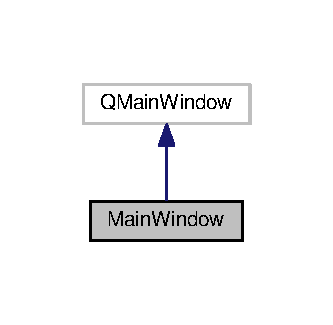
\includegraphics[width=160pt]{classMainWindow__inherit__graph}
\end{center}
\end{figure}


Collaboration diagram for Main\+Window\+:\nopagebreak
\begin{figure}[H]
\begin{center}
\leavevmode
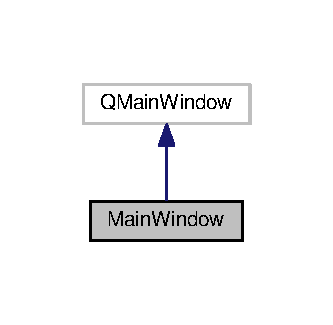
\includegraphics[width=160pt]{classMainWindow__coll__graph}
\end{center}
\end{figure}
\subsection*{Public Member Functions}
\begin{DoxyCompactItemize}
\item 
\hyperlink{classMainWindow_a8b244be8b7b7db1b08de2a2acb9409db}{Main\+Window} (Q\+Widget $\ast$parent=0)\hypertarget{classMainWindow_a8b244be8b7b7db1b08de2a2acb9409db}{}\label{classMainWindow_a8b244be8b7b7db1b08de2a2acb9409db}

\begin{DoxyCompactList}\small\item\em имя таблицы для базы \end{DoxyCompactList}\end{DoxyCompactItemize}


The documentation for this class was generated from the following files\+:\begin{DoxyCompactItemize}
\item 
mainwindow.\+h\item 
mainwindow.\+cpp\end{DoxyCompactItemize}

%--- End generated contents ---

% Index
\backmatter
\newpage
\phantomsection
\clearemptydoublepage
\addcontentsline{toc}{chapter}{Index}
\printindex

\end{document}
